
\section{方法}
\subsection{optparseとThorの比較}
今回の研究対象のhikiutilsは,optparseというコマンドライン解析ライブラリで実装されている.
本研究ではこの代替ライブラリとしてThorの採用を検討した.
本章の最初では,FizzBuzzという簡単なコードを例にoptparseとThorにより作成するコマンドライン解析コードの比較を行う.FizzBuzzはThorの使い方を解説した記事\cite{1-2}で紹介されている.比較しやすくするためoptparseでFizzBuzzを新たに実装した.

\subsubsection{Thor}
Thorとは,コマンドラインツールの作成を支援するライブラリのことである.gitやbundlerのようにサブコマンドを含むコマンドラインツールを簡単に作成することができる\cite{1-2}.

Thorの基本的な流れとしては

\begin{enumerate}
\item Thorを継承したクラスのメソッドがコマンドになる
\item クラス.start(ARGV)でコマンドラインの処理をスタートする
\end{enumerate}
である\cite{1-2}.

startに渡す引数が空の場合,Thorはクラスのヘルプリストを出力する.また,Thorはサブコマンドやサブサブコマンドも容易に作ることができる.

以下に示したコードがThorで記述されたfizzbuzzである.
\begin{lstlisting}[style=customRuby,basicstyle={\scriptsize\ttfamily}]
module Fizzbuzz                                                   
  class CLI < Thor

    desc 'fizzbuzz', 'Get fizzbuzz result from limit number'
    def fizzbuzz(limit)
      print Fizzbuzz.fizzbuzz(limit).join(',')
      exit
    end

    desc 'version', 'version'
    def version
      puts Fizzbuzz::VERSION
    end
  end
end
\end{lstlisting}
このコードもoptparseのfizzbuzzと同様fizzbuzzとversionのコマンドを実行させる.

\paragraph{fizzbuzzメソッド,versionメソッド}
descでコマンド一覧で表示させるコマンド名と説明を書く.メソッド内ではそれぞれのコマンドの処理内容が書かれている.

\subsubsection{optparse}
optparseとは,getoptよりも簡便で,柔軟性に富み,かつ強力なコマンドライン解析ライブラリである.optparseでは,より宣言的なスタイルのコマンドライン解析手法,すなわちOptionParserのインスタンスでコマンドラインを解析するという手法をとっている.これを使うと,GNU/POSIX構文でオプションを指定できるだけでなく,使用法やヘルプメッセージの生成も行える\cite{1-3}.利用頻度はあまり高くないが古くから開発され,使用例が広く紹介されている.

optparseの基本的な流れとしては

\begin{enumerate}
\item OptionParserオブジェクトoptを生成する
\item オプションを取り扱うブロックをopt.onに登録する
\item opt.parse(ARGV)でコマンドラインを実際にparseする
\end{enumerate}
である.

OptionParserはコマンドラインのオプション取り扱うためのクラスであるためオブジェクトoptを生成されopt.onにコマンドを登録することができる.しかし,OptionParser\#onにはコマンドが登録されているだけであるため,OptionParser\#parseが呼ばれた時,コマンドラインにオプションが指定されていれば実行される.optparseにはデフォルトとして--helpと--versionオプションを認識する\cite{1-4}.

以下に示したコードがoptparseで記述したfizzbuzzである.
\begin{lstlisting}[style=customRuby,basicstyle={\scriptsize\ttfamily}]
module Fizzbuzz
  class Command

     def self.run(argv)
       new(argv).execute
     end

     def initialize(argv)
       @argv = argv
     end

     def execute
       options = Options.parse!(@argv)
       sub_command = options.delete(:command)
       case sub_command
            when 'fizzbuzz'
              fizzbuzz(options[:id])
            when 'version'
              version
            end
     end

     def fizzbuzz(limit_number)
       (0..limit_number).map do |num|
         if (num % 15).zero? then print 'FizzBuzz'
         elsif (num % 5).zero? then print 'Buzz'
         elsif (num % 3).zero? then print 'Fizz'
         else print num.to_s
         end
         print ' '
       end
     end

     def version
       puts Fizzbuzz::VERSION
       exit
     end
  end
end
\end{lstlisting}
このコードはfizzbuzzとversionをコマンドとして実行できる.

\paragraph{runメソッド}
コマンド実行を行うためのメソッドであり,argv配列を代入することでexecuteメソッドを実行する.

\paragraph{initializeメソッド}
初期化を行うメソッドである.
\begin{quote}\begin{verbatim}
@argv = argv
\end{verbatim}\end{quote}
こうすることでargvをクラス内で利用できるようにする.

\paragraph{executeメソッド}
上記でoptparseではopt.onにコマンドを登録する必要があると説明したが,opt.onで登録できるものはハイフンがついたコマンドだけであり,ハイフンなしのコマンドの登録はこのようになる.

argv配列の解析を行うOptions.parse!(@argv)をoptionsに代入して解析を行いsub\_commandに代入する.sub\_commandがfizzbuzzであればfizzbuzz(options[:id])メソッドを実行,versionであればversionメソッドを実行する.

\paragraph{fizzbuzzメソッド}
引数としてlimit\_numberを受け取り,0〜limit\_numberまでの数字を繰り返す.numが15であればFizzbuzzを表示,5であればBuzzを表示,3であればFizzを表示,それ以外は数字を表示し,その後に空白を表示する.

\paragraph{versionメソッド}
fizzbuzzのバージョンを表示する.

\subsection{既存のhikiutilsのコマンド解説}
既存のhikiutilsはコマンド解析ライブラリのoptparseを用いて,コマンドの処理を行っている.
optparseの特徴は,「コマンドの登録,実行method」に分けて記述することが期待されている.
また,CLIの起動の仕方が特徴的である.この二つを取り出して,動作とコードを説明する.

\subsubsection{コマンドの登録と実行メソッド}
optparseのコマンド登録と実行メソッドの呼び出し関係は図\ref{fig:005}の通りである.

\begin{figure}[htbp]\begin{center}
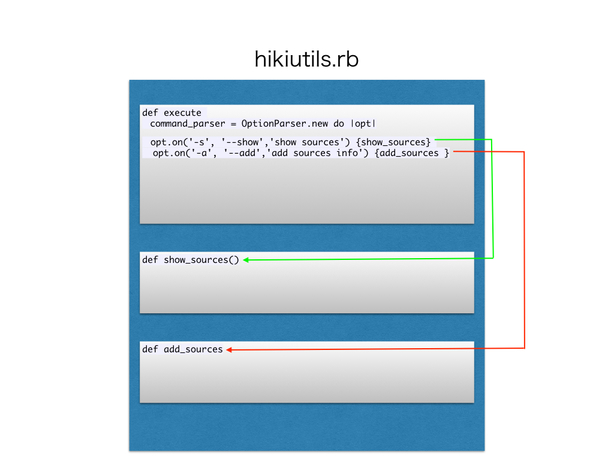
\includegraphics[width=12cm,bb= 0 0 737 553]{../figs/./hikiutils_yamane.005.jpg}
\caption{コマンドの登録と実行メソッドの対応.}
\label{fig:005}
\label{default}\end{center}\end{figure}
optparseでは以下の通り,コマンドの登録と実行が行われる.

\begin{enumerate}
\item OptionParserオブジェクトoptを生成
\item optにコマンドを登録
\item 入力されたコマンドの処理のメソッドへ移動
\end{enumerate}
この実装コードは次の通りである.
\begin{lstlisting}[style=customRuby,basicstyle={\scriptsize\ttfamily}]
    def execute
      @argv << '--help' if @argv.size==0
      command_parser = OptionParser.new do |opt|
        opt.on('-v', '--version','show program Version.') { |v|
          opt.version = HikiUtils::VERSION
          puts opt.ver
        }
        opt.on('-s', '--show','show sources') {show_sources}
        opt.on('-a', '--add','add sources info') {add_sources }
        opt.on('-t', '--target VAL','set target id') {|val| set_target(val)}
        opt.on('-e', '--edit FILE','open file') {|file| edit_file(file) }

        ...省略...

      end
      begin
        command_parser.parse!(@argv)
      rescue=> eval
        p eval
      end
      dump_sources
      exit
    end    
    
    def show_sources()
      printf("target_no:%i\n",@src[:target])
      printf("editor_command:%s\n",@src[:editor_command])

      ...省略...

    end

    以下略

\end{lstlisting}
optparseではOptionParserオブジェクトoptの生成を行い,コマンドをoptに登録することでコマンドを作成することができる.しかし,これはコマンドを登録しているだけでコマンドの一覧ではこれを表示することができるが,コマンドの実行を行うためには実行を行うためのメソッドを作成する必要がある.optparseでのコマンドの実行はoptで登録されたコマンドが入力されることでそれぞれのコマンドの処理を行うメソッドに移動し処理を行う.しかし,このコマンド登録はハイフンを付けたコマンドしか登録ができず,ハイフンなしのコマンド登録はまた別の手段でやらなくてはいけない.

\subsubsection{CLIの実行プロセス}
optparseを用いた場合のCLIの実行プロセスは図\ref{fig:007}の通りとなる.

\begin{figure}[htbp]\begin{center}
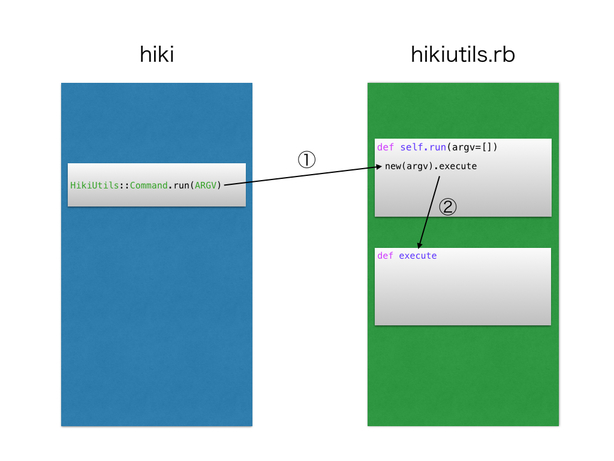
\includegraphics[width=12cm,bb= 0 0 737 553]{../figs/./hikiutils_yamane.007.jpg}
\caption{CLIの実行プロセス.}
\label{fig:007}
\label{default}\end{center}\end{figure}
CLIの実行プロセスは次の通りとなる.

\begin{enumerate}
\item HikiのHikiUtils::Command.run(ARGV)でhikiutils.rbのrunメソッドを呼ぶ
\item new(argv).executeでexecuteメソッドが実行される
\end{enumerate}
optparseではHikiutils::Command.run(ARGV)で実行され,requireで呼び出されたhikiutils.rbのrunメソッドが実行される.そこでコマンドを登録しているexecuteメソッドへ移動し入力したコマンドと対応させる.そして,対応したコマンドの処理が行われるメソッドに移動することで実行される.このようにoptparseでは実行を行うためのメソッドが必要である.

\subsubsection{コード}
optparseの呼び出し側のexe/hikiのコードは次の通りである.
\begin{lstlisting}[style=customRuby,basicstyle={\scriptsize\ttfamily}]
#!/usr/bin/env ruby                                                             

require "hikiutils"

HikiUtils::Command.run(ARGV)
\end{lstlisting}
「require "hikituils"」ではlib/hikiutils.rbを読み出してくることを期待している.
これはgemspecファイルでlibへのロードパスの記述がされているため,hikiutils.rbを参照することができる.
「Hikiuils::Command.run(ARGV)」ではlib/hikiutils.rbのHikiUtilsモジュールCommandクラスのrunメソッドを実行する記述が成されている.

また呼び出される側のlib/hikiutils.rbのrunおよびexecute部のコードは次の通りとなる.
\begin{lstlisting}[style=customRuby,basicstyle={\scriptsize\ttfamily}]
    def self.run(argv=[])
      print "hikiutils: provide utilities for helping hiki editing.\n"
      new(argv).execute
    end

    def execute
      @argv << '--help' if @argv.size==0
      command_parser = OptionParser.new do |opt|
        opt.on('-v', '--version','show program Version.') { |v|
          opt.version = HikiUtils::VERSION
          puts opt.ver
        }
        opt.on('-s', '--show','show sources') {show_sources}
        opt.on('-a', '--add','add sources info') {add_sources }
        opt.on('-t', '--target VAL','set target id') {|val| set_target(val) }
        opt.on('-e', '--edit FILE','open file') {|file| edit_file(file) }
        opt.on('-l', '--list [FILE]','list files') {|file| list_files(file) }
        opt.on('-u', '--update FILE','update file') {|file| update_file(file) }
        opt.on('-r', '--rsync','rsync files') {rsync_files}
        opt.on('--database FILE','read database file') {|file| db_file(file)}
        opt.on('--display FILE','display converted hikifile') {|file| display(f\
ile)}
        opt.on('-c', '--checkdb','check database file') {check_db}
        opt.on('--remove FILE','remove file') {|file| remove_file(file)}
        opt.on('--move FILES','move file1,file2',Array) {|files| move_file(file\
s)}
        opt.on('--euc FILE','translate file to euc') {|file| euc_file(file) }
        opt.on('--initialize','initialize source directory') {dir_init() }
      end
      begin
        command_parser.parse!(@argv)
      rescue=> eval
        p eval
      end
      dump_sources
      exit
    end  
\end{lstlisting}
runメソッドでは「hikiutils: provide utilities for helping hiki editing.」を表示させ,executeメソッドを実行させる.
executeメソッドでは最初に「@argv << '--help' if @argv.size==0」と記述する.これはもしargv配列の中身が空であればargv配列に'--help'を代入する.「command\_parser = OptionParser.new do |opt|」ではOptionParserオブジェクトがoptを生成しコマンドを登録していき,command\_parserに代入する.そして,「command\_parser.parse!(@argv)」では@argvにある文字列をcommand\_parserでparseする.つまり,ここでは入力されたコマンドを解析し,登録されたコマンドと一致すればその処理が行われる.もし,一致しなければevalメソッドで表示する.

